% Drafted against audit/outline.md §6. The outline's figures predate the
% disclosed-window rerun and are superseded throughout: the recalibrated book
% averages 44.7 rather than 42.8, the fixed book 41.6 with sd 6.33, and the
% frontier is now stated against the disclosed standard deviation itself.
% The outline's §6 block is corrected in the same commit as this draft.
%
% Evidence: diversification_comparison.csv, robustness_sign_variants.csv,
% backtest_results.csv, hash-recorded in audit/evidence_freeze.csv at commit
% 8c4a5cf7.

\section{Results}\label{sec:results}

\subsection{The level}

The level reproduces. Table~\ref{tab:results} sets the disclosed series beside
both proxy books. Over the ten years Goldman's diversification effect averages
42.0\% of summed category VaR; the book sized once on 2019 and then left alone
averages 41.6\%. A Welch test does not separate the two ($t = -0.20$,
$p = 0.84$), which is the appropriate way to report the agreement: the
difference is small, but with ten annual observations and a proxy mean whose
95\% interval runs from 37.1 to 46.1, the precision implied by quoting it to a
decimal place is not there. The book resized each year to the disclosed split
averages 44.7\%, which overshoots and sits just outside the disclosed range of
39.0 to 45.5 on the high side.

% Generated by build/make_tables.py from diversification_comparison.csv. Do not edit.

\begin{table}[tbp]
\centering
\small
\caption{The disclosed diversification effect against the proxy book, FY2016--FY2025}
\label{tab:results}
\begin{tabular}{@{}lrrrr@{}}
\toprule
 & \multicolumn{3}{c}{Diversification effect (\% of summed)} & Total VaR \\
\cmidrule(lr){2-4}
Year & Goldman & Resized yearly & Fixed since 2019 & error (\%) \\
\midrule
2016 & 41.7 & 53.9 & 49.3 & -21.0 \\
2017 & 39.3 & 47.6 & 46.1 & -13.7 \\
2018 & 41.2 & 44.8 & 43.2 & -6.1 \\
2019 & 41.7 & 45.1 & 45.1 & -5.8 \\
2020 & 44.4 & 49.6 & 45.5 & -9.4 \\
2021 & 39.0 & 48.1 & 45.8 & -14.9 \\
2022 & 45.5 & 43.6 & 42.4 & +3.3 \\
2023 & 41.1 & 37.7 & 34.5 & +5.7 \\
2024 & 43.6 & 39.1 & 32.3 & +8.0 \\
2025 & 43.0 & 37.9 & 31.9 & +9.1 \\
\midrule
Mean & 42.0 & 44.7 & 41.6 & \\
Std.\ dev. & 2.08 & 5.35 & 6.33 & \\
\bottomrule
\end{tabular}
\notetext{The diversification effect as a share of summed category VaR, by Goldman's own definition. \emph{Resized yearly} is the book recalibrated to each year's disclosed split; \emph{fixed since 2019} is sized once on 2019 and left alone. The final column is the error in the fixed book's total VaR against the disclosed total, which changes sign in 2022. The dollar level of the book is a normalisation, so that column measures the consequence of the diversification gap rather than a sizing error: Table~\ref{tab:sizing} shows the sizing is exact.}
\end{table}


That the fixed book matches more closely than the recalibrated one is worth a
sentence, because the opposite would be the natural expectation. Recalibration
forces each sleeve's standalone VaR onto the disclosed figure every year, which
removes the exposure mix from the comparison; it does not remove it from the
correlation structure, because changing sleeve sizes changes how the sleeves
offset one another in the joint tail. The fixed book has no such annual
intervention, and over a decade its level happens to land closer. Neither
result should be over-read: both are within a few points of a figure the
engine was never told, and the agreement is the finding rather than the
difference between the two books.

This result corroborates rather than discovers.
\citet{perignon2010diversification} found that disclosed diversification
effects sit close to independently estimated ones, on four US banks and
quarterly data ending in early 2007. The same holds here, on a different bank,
a different decade and a different method (public factors and a proxy book
rather than their estimation), which is what makes it corroboration worth
reporting: the finding survives a change of almost everything except the
question.

\subsection{The steadiness}

The steadiness does not reproduce, and the failure is directional rather than
noisy.

Goldman's series has a standard deviation of 2.08 percentage points across the
ten years. The fixed book's is 6.33, three times as large, and the difference
is not an artefact of small samples: a variance-ratio test gives $F = 9.26$ on
$(9,9)$ degrees of freedom with $p = 0.0028$, and Bartlett's test agrees.
Levene's test, which is robust to departures from normality and the safer
choice at this sample size, is borderline at $p = 0.055$. The parametric
result is reported with the robust one rather than instead of it.

The two series also move differently over the decade. Goldman's mean for
2021--2025 is 0.8 points above its mean for 2016--2020; the fixed book's is 8.5
points below, and the book finishes the sample 17.4 points lower than it
started. Figure~\ref{fig:overtime} shows the three series together, and the
shape is the result: a flat disclosed line and two proxy lines that track it
until 2022 and then fall away from it.

No regression trend or $p$-value is quoted for these movements, and the reason
is worth stating because it constrains what any study of this kind can claim.
The proxy's annual values are computed from overlapping five-year scenario
windows: with about 230 trading days a year inside a 1{,}260-day window,
consecutive annual figures share roughly 82\% of the data that produces them.
Least-squares standard errors on ten such observations assume an independence
the construction rules out, and would overstate the significance of any trend
by a wide margin. The decline is large and visible; it is not something a
significance test on this sample can certify.

\begin{figure}[tbp]
\centering
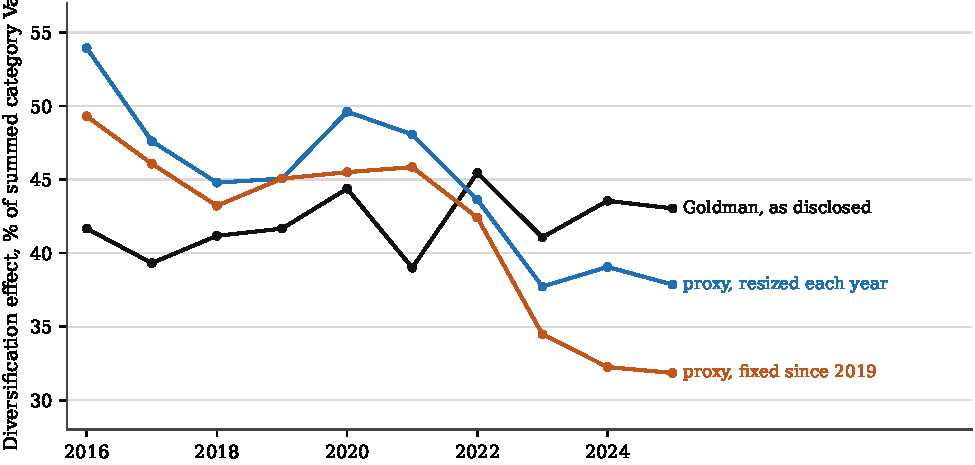
\includegraphics[width=\linewidth]{figures/diversification_over_time}
\caption{The disclosed diversification effect and the proxy book, FY2016--FY2025.
Goldman's series is flat across a decade containing a pandemic, a zero-rate
period and more than 500 basis points of policy tightening. Both proxy books
track it until 2022 and then decline, as the five-year scenario window fills
with the 2022 correlation regime and does not empty again.}
\label{fig:overtime}
\end{figure}

The mechanism is visible in the final column of Table~\ref{tab:results}. The
error in the fixed book's total VaR changes sign in 2022. Before then the proxy
over-diversifies, understating total VaR by as much as 21.0\%; afterwards it
under-diversifies, overstating total VaR by up to 9.1\%. The turn is the
equity--bond correlation moving positive in the inflation regime, which removes
the main diversifier available to a directional book. Goldman's ratio went
\emph{up} that year, to its sample maximum of 45.5\%.

The decline afterwards is a property of a long window on a static book. Once
2022 enters a five-year scenario set it stays there until 2027, so the measured
correlation structure keeps the inflation regime in view long after the market
has left it. Appendix~\ref{sec:appendix_c} cuts the same daily output into
market regimes, where the effect is starkest: the measured diversification
falls from 44.8\% in the calm years to 32.1\% in 2024--2025, on a book that
did not change. A dealer repositioning daily has no such ratchet, and
Section~\ref{sec:assumptions} shows that shortening or reweighting the window
does not rescue the result.

\subsection{Amplitude against persistence}

Goldman publishes the diversification effect twice: averaged over the year's
daily values, and as a period-end snapshot. Everything above compares the
average daily series, which is the measure the firm leads with. Comparing the
other one separates two things the first comparison conflates --- how far the
ratio moves, and whether those movements persist --- and the separation is
informative enough to change how the gap should be described.

% Generated by build/make_tables.py from gs_var_average_daily.csv, gs_var_period_end.csv and var_fixed_book_daily.csv. Do not edit.

\begin{table}[tbp]
\centering
\small
\caption{Amplitude and persistence: the two disclosed measures of the diversification effect against their proxy analogues}
\label{tab:amplitude}
\begin{tabular}{@{}lrrlrr@{}}
\toprule
 & & Std. & & Change, first & Lag-1 \\
Series & Mean & dev. & Range & half to second & autocorr. \\
\midrule
Goldman, average daily & 42.03 & 2.08 & 39.0--45.5 & +0.8 & -0.47 \\
Goldman, period-end & 38.21 & 6.72 & 28.6--48.6 & +8.6 & +0.07 \\
\addlinespace
Proxy, average daily & 41.60 & 6.33 & 31.9--49.3 & -8.5 & +0.88 \\
Proxy, final day of year & 40.62 & 6.68 & 30.6--47.8 & -10.2 & +0.90 \\
\bottomrule
\end{tabular}
\notetext{All figures are the diversification effect as a percentage of summed category VaR across the ten fiscal years, so each column rests on ten observations and none is precisely estimated. \emph{Change} is the mean of 2021--2025 less the mean of 2016--2020. \emph{Lag-1 autocorr.} is the correlation between consecutive annual values: negative indicates a series that returns toward its mean, positive one that carries its level forward. Neither disclosed series shows positive persistence --- the average daily series is $-0.47$ and the period-end series is essentially zero --- while both proxy series sit near $+0.9$. That contrast, rather than any difference in spread, is what Section~\ref{sec:results} rests on. No trend test is reported: the proxy's annual values are computed from overlapping five-year windows and share about 82\% of their scenario set with their neighbours, so a regression on them would understate its own standard errors.}
\end{table}


Table~\ref{tab:amplitude} sets both disclosed measures beside their proxy
analogues. The first thing it shows is that Goldman's ratio is not a stable
quantity. Measured period-end it has a standard deviation of 6.72 percentage
points and a range of 28.6 to 48.6, against 2.08 and 39.0 to 45.5 for the
average daily series. What is steady in the disclosures is the annual mean, not
the ratio.

The decisive column is the last one. The lag-1 autocorrelation of a series,
the correlation between consecutive annual values, distinguishes a quantity
that returns toward its mean from one that carries its level forward, and it
requires no model and no trend. Neither disclosed series shows positive
persistence: the average daily series is $-0.47$ and the period-end series is
essentially zero at $+0.07$. Both proxy series sit near $+0.9$. Whatever each
series does in a given year, Goldman's does not carry forward and the proxy's
does.

That is the finding, and it is sharper than a comparison of spreads. The proxy
does not fail to vary, nor vary too much; it fails to come back. Reading
Figure~\ref{fig:overtime} again with that in mind, the proxy lines do not
simply wobble more than the disclosed line; they leave and stay left.

The spread comparison corroborates this without carrying it. Measured
period-end against period-end the proxy's standard deviation is 6.68 against
Goldman's 6.72, which on inspection looks like an exact match and on
examination is not: each is estimated from ten observations, and the 95\%
confidence interval on the \emph{ratio} of the two runs from 0.50 to 2.02. The
defensible statement is that the two amplitudes are statistically
indistinguishable ($F = 1.01$, $p = 0.98$), which is weaker than reproduction
and is not evidence of equality. What the comparison does establish is that the
gap between the two average daily series is not simply a matter of the proxy
being more volatile, because measured alike the volatilities cannot be told
apart.

Two further qualifications. Each period-end figure is a single trading day, so
those rows rest on ten single-day observations and year-end snapshots may carry
balance-sheet effects an average does not. And the proxy's final trading day is
the last day of the aligned calendar rather than Goldman's fiscal period end.

\subsection{The configuration space}

A single calibration proves little, because the direction of each sleeve is not
disclosed and the diversification effect depends on those directions more than
on anything else in the specification. All sixteen sign combinations were
therefore run on the fixed book, and Figure~\ref{fig:frontier} plots each one's
decade-average level against its year-to-year standard deviation.

\begin{figure}[tbp]
\centering
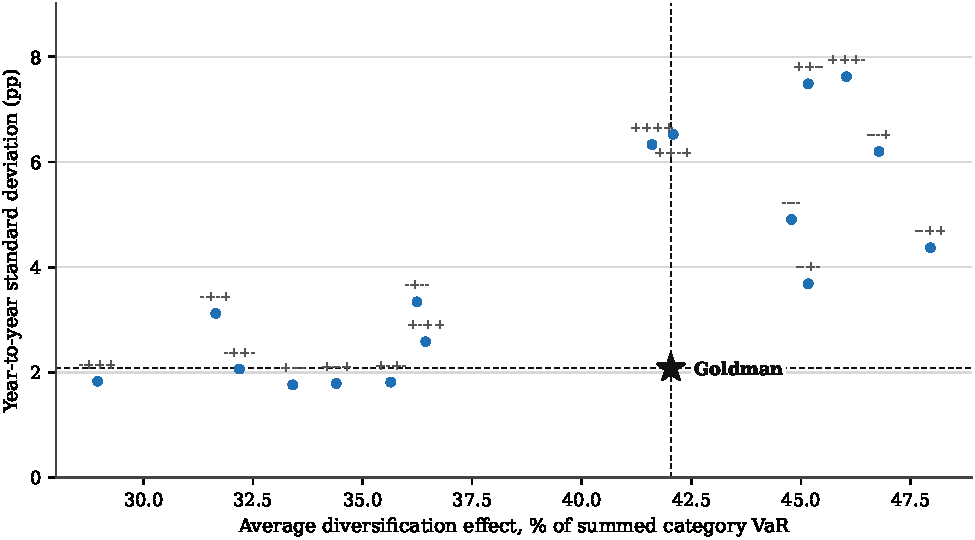
\includegraphics[width=\linewidth]{figures/stability_frontier}
\caption{Level against steadiness for all sixteen sleeve-sign configurations,
with Goldman's own position marked. Signs are in the order interest rates,
equity, currency, commodity. The dashed lines are Goldman's average level and
its year-to-year standard deviation; the quadrant below and to the right of
their intersection --- at least as steady as the disclosure, and at least as
high --- contains no configuration.}
\label{fig:frontier}
\end{figure}

Taking the disclosed standard deviation itself as the bar rather than a round
number chosen afterwards: five of the sixteen configurations are at least as
steady as Goldman's 2.08, and the highest of those averages 35.64\%, six points
below the disclosure. Eight average 40\% or more, and the steadiest of those
varies by 3.68 points a year, about 77\% more than Goldman. No configuration
achieves both.

This is a descriptive bound on what the engine can produce, and it should be
read as one rather than as a test. Every standard deviation in
Figure~\ref{fig:frontier} is estimated from ten annual observations and
carries a confidence interval spanning roughly a factor of two and a half in
each direction; the steadiest configuration's 3.68 and Goldman's 2.08 are not
separated by anything a formal comparison would certify. The sixteen
configurations are not independent draws either, since they share the same
factor data and differ only in sleeve signs, and the figures quoted are the
selected extremes across them, with no adjustment for that selection.

What the bound does establish is the shape of the trade-off. Within this
engine, moving a configuration toward Goldman's level moves it away from
Goldman's steadiness, across the whole sign space rather than at one point.
That is what makes the gap hard to explain away as a bad choice of signs: the
better choice would have to lie outside the space, and the space is complete.

\subsection{Backtest behaviour}

The engine's own coverage is reported here because it bears on how much weight
the diversification result can carry, and because it replicates a known finding
on a new sample. Table~\ref{tab:backtest} gives the four variants.

% Generated by build/make_tables.py from backtest_results.csv. Do not edit.

\begin{table}[tbp]
\centering
\footnotesize
\setlength{\tabcolsep}{4pt}
\caption{Backtest results on the fixed book}
\label{tab:backtest}
\begin{tabular}{@{}lllrrrrrrl@{}}
\toprule
Model & Conf. & Period & Days & Exc. & Rate (\%) & Kupiec & Indep. & Joint & Zone \\
\midrule
Historical simulation & 95\% & 2016-2025 & 2,293 & 160 & 6.98 & $<$0.0001 & $<$0.0001 & $<$0.0001 & red \\
Historical simulation & 95\% & 2020-2025 & 1,373 & 127 & 9.25 & $<$0.0001 & $<$0.0001 & $<$0.0001 & red \\
\addlinespace
Volatility weighted & 95\% & 2016-2025 & 2,293 & 117 & 5.10 & 0.822 & 0.110 & 0.272 & yellow \\
Volatility weighted & 95\% & 2020-2025 & 1,373 & 70 & 5.10 & 0.868 & 0.213 & 0.454 & yellow \\
\addlinespace
Historical simulation & 99\% & 2016-2025 & 2,293 & 45 & 1.96 & $<$0.0001 & $<$0.0001 & $<$0.0001 & red \\
Historical simulation & 99\% & 2020-2025 & 1,373 & 44 & 3.20 & $<$0.0001 & $<$0.0001 & $<$0.0001 & red \\
\addlinespace
Volatility weighted & 99\% & 2016-2025 & 2,293 & 19 & 0.83 & 0.395 & 0.573 & 0.594 & green \\
Volatility weighted & 99\% & 2020-2025 & 1,373 & 13 & 0.95 & 0.842 & 0.618 & 0.866 & green \\
\bottomrule
\end{tabular}
\notetext{Kupiec, Indep.\ and Joint are $p$-values for the proportion-of-failures, independence and conditional coverage tests. \emph{Zone} is the worst Basel traffic-light zone reached on any rolling 250-day window, computed at the confidence level of the row rather than at the published 99\% boundaries. The book is sized once on 2019, so the 2020--2025 rows are out of sample with respect to sizing.}
\end{table}


Plain historical simulation at the disclosed five-year window fails, and fails
on count as well as on arrangement: 160 exceptions in 2{,}293 days is a rate of
6.98\% against a nominal 5\%, which Kupiec rejects below any conventional
level, and the rate rises to 9.25\% from 2020. The failures cluster badly ---
70 of them fall in 2022 alone, out of 230 trading days --- and the model spends
18.2\% of days in the Basel red zone, peaking at 73 exceptions in a 250-day
window against a red threshold of 27.

Restating the scenario set in current volatility units repairs it. The
\citet{hullwhite1998} variant is not rejected by any of the three tests at
either confidence level: at 99\% it stays in the green zone throughout, peaking
at 4 exceptions in a 250-day window against a yellow threshold of 5. The
exception rate falls from 6.98\% to 5.10\% at 95\%, and the independence
statistic from 37.7 to 2.6.

This reproduces \citet{obrien2017evaluation} on a proxy book and a newer
sample. They found bank VaR exceedances excessive and clustered in the crisis,
and a conditional-volatility benchmark achieving lower exceedance rates without
clustering; the same pattern appears here, with the long disclosed window
standing in for the slow adjustment they document.

One comparison must be read carefully. Goldman disclosed 10 exceptions at 95\%
across the ten years, roughly 0.40\% of trading days against a nominal 5\%. A
literal coverage test on that count would reject calibration at any level, and
the rejection would be meaningless, because the two measurements are not the
same quantity. Goldman compares VaR against \emph{net revenues}, which include
intraday market-making income that is positive far more often than not; the
filings say so, and say it is why exceptions are rarer than the confidence
level implies. The proxy book has no client flow and no bid--offer spread, so
its profit and loss is a clean mark on a static position. The distance between
0.40\% and 5\% is an indication of how much the revenue cushion is worth, and
it is large, but it is not evidence that either model is miscalibrated. The
comparison is reported in Appendix~\ref{sec:appendix_a} and is not used
anywhere in this paper's conclusions.
